\chapter{The International Linear Collider}
\label{ILC}
\begin{chapterabstract}
For answering the fundamental questions of mankind, it is necessary to understand the world in great detail.
In order to confirm theories in particle physics, or to disproof them, it is often important to be able to measure the qualities of particles or their interactions to the tenth decimal place or better.
For measurements being done in high-energy particle colliders, such precisions can only be reached in linear lepton colliders, as has already been shown in Chapter~\ref{LinearColliderPhysics}.
The following sections will present a new design for such a collider of the precision frontier: the International Linear Collider (ILC). 
Its proposed layout, the possible construction sites, the detectors, and finally the physics motivation for such a capable accelerator will be explained.
\end{chapterabstract}
\newline

The International Linear Collider (ILC) is a proposed linear \positron\electron collider with state of the art technologies for the detectors and the machine, so that high precision measurements will be possible.

\section{Motivating the layout}
\label{ILC:layout}
The ILC was originally designed to collide electron and positron beams with a center-of-mass energy of \SI{500}{\GeV} in the first stage of operation.
Because of political developments and the request in 2017 to reduce the construction cost, the first stage collision energy was reduced to \SI{250}{\GeV}.
Due to the fact that linear colliders can be extended in length, the beam energies can linearly be increased.
Therefore, the ILC has the possibility to upgrade the machine to higher energies later on.

\subsection{The Layout}
Figure~\ref{fig:ILC_Layout} shows the schematic layout of the ILC.
\begin{figure}
\centering
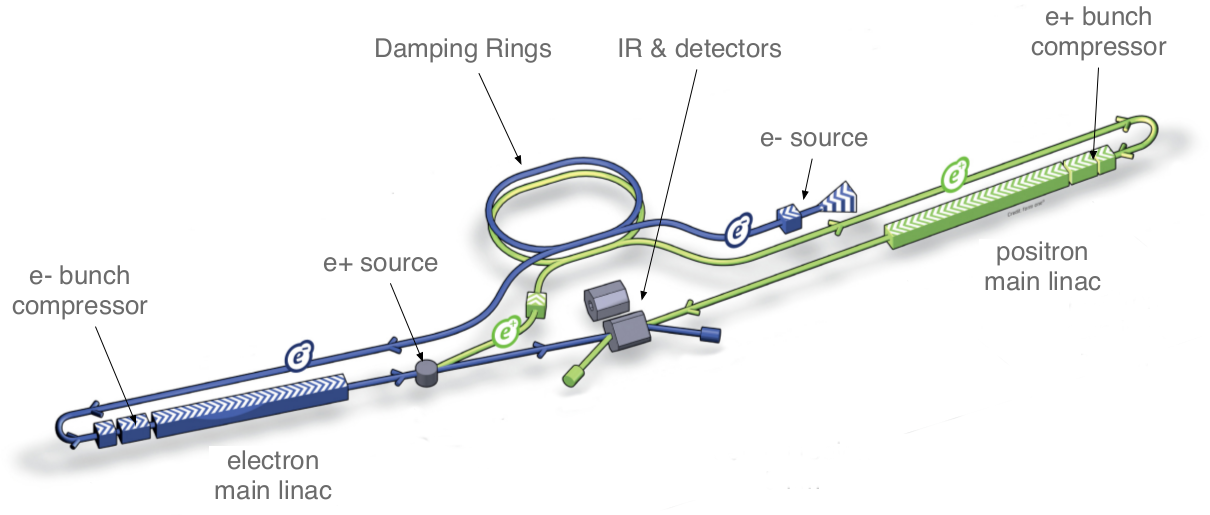
\includegraphics[width=\textwidth]{Figures/ILC_layout_edited.png}
\caption[Schematic layout of the ILC]{Schematic layout of the ILC~\cite[cf. p. 9]{TDR1}}
\label{fig:ILC_Layout}
\end{figure}\todo{I have edited this figure slightly -> how to do the citation correctly?}
The electrons are produced by a GaAs photocathode in a DC electron gun.~\cite[p. 13]{TDR32}
By shining a circularly polarized laser on the electron beam, one reaches a beam polarization of at least 80\,\%, i.e. more than 80\,\% of all electrons will be left-handed\footnote{For a left-handed particle, its spin and its momentum are antiparallel, pointing in opposite directions.}:
\begin{equation}
 P_e = \frac{N_L-N_R}{N_L+N_R} > 0.8
\end{equation}
The positron source consists of an undulator and a conversion target.
In an undulator, several dipole magnets are placed in a line in such a way that their polarity alternates periodically (see Figure~\ref{fig:Undulator}).\todo{I have edited this figure slightly -> how to do the citation correctly?}
For the creation of the positrons, the actual electron beam is used, which is guided through the  \SI{231}{\meter} long undulator after being pre-accelerated.
By doing so, the electrons are deflected several times and emit synchrotron radiation photons, as explained in Chapter~\ref{AccPhysics:Linear-Circular}.
The high-energy photons are then converted in the \SI{7}{\milli\meter} thick titanium-alloy conversion target, where \positron \electron pairs are produced due to pair production.
The positrons are captured and form the positron beam.
Due to the usage of an undulator and the conversion from photons, the positrons will have a polarization of 30\,\%.~\cite[p. 14]{TDR32}
The whole process leads to a positron yield of 1.5 positrons per original beam electron passing through the undulator.~\cite{Ushakov}
\begin{figure}
\centering
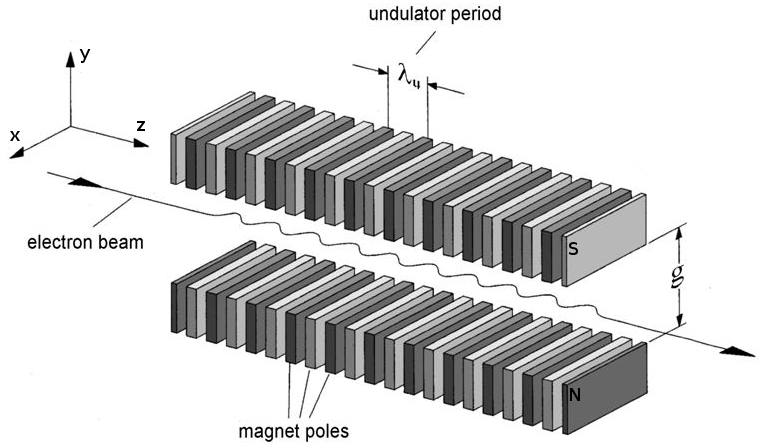
\includegraphics[width=0.8\textwidth]{Figures/Undulator_edited.png}
\caption[Schematic layout of an undulator]{Schematic of an electron beam traveling through an undulator with dipole magnets in alternating order.~\cite[cf. p. 41]{Wille}}
\label{fig:Undulator}
\end{figure}
\\The polarized positrons then continue along the positron line which is from that point on equivalent to the electron line.
Since the electrons and positrons have a large emittance when they originate from their sources, their momentum and beam size have to be condensed.
This is done in the damping rings (DR), which have a circumference of \SI{3.2}{\kilo\meter}.~\cite[p. 14]{TDR32}
As discussed several times before, the beams will emit synchrotron radiation when they are deflected in a magnetic field.
Exactly this is desired in the damping rings in order to ``cool'' the beams, i.e. to reduce their momentum due to the emission of light.
In a second step the beams are then accelerated again which increases their momentum in the desired direction.
The result is a high quality beam with small beam emittance.\\
After passing the damping rings, the electron and positron beams are compressed into bunches by a two-stage compressor system.
Here, the bunch length is reduced from several millimeters to \SI{300}{\micro\meter}.
In both compressor systems, RF cavities are used together with undulators, which compact the beam momentum.
The usage of two separate systems allows more flexibility in the operation, e.g. to reduce the beam length below \SI{300}{\micro\meter}.~\cite[p. 124]{TDR32}\\
Subsequent to that, the bunches are injected into the main linear accelerator structures (main linacs).
The main linacs have a length of \SI{5}{\kilo\meter}, and use superconducting RF cavities which are shown in Figure~\ref{fig:Tesla_Cavity} in Chapter~\ref{AccPhysics:Principles}. 
For the machine upgrade to \SI{500}{\GeV}, the linacs can be extended in length.
Since these exact cavities are already in use for the European XFEL (X-Ray Free-Electron Laser) at Deutsches Elektronen-Synchrotron (DESY) in Hamburg, their high performance has been demonstrated.
It has been shown that they have an average accelerating gradient of \SI{31.5}{MV/m}, and that they can be operated with a frequency of \SI{1.3}{\giga\hertz}.~\cite{Walker}\\
The Beam Delivery System (BDS), which has an overall length of about \SI{4.4}{\kilo\meter}, transports the bunches from the linacs to the Interaction Point (IP).
In the BDS, the beams are focused to nanometer size by the Final-Focus (FF) system.
The Final-Focus system is a crucial part of the ILC program.
Only with nanometer-sized beams, the ILC can reach luminosities comparable to or beyond the Large Hadron Collider (LHC) at CERN.
To demonstrate the feasibility of nanometer-scale beams, a test facility was build that is a small scale prototype of the FF system for the ILC: the Accelerator Test Facility (ATF2), which will be presented in more detail in Section~\ref{ATF2}.
The BDS system does not only contain the quadrupoles and sextupoles in FF system, but also various feedback diagnostics and beam-halo collimators for removing the halo of particles around the beam core in order to reduce the beam background at the IP. 
Additionally, shielding systems are installed at various locations along the BDS line, again in order to keep the background level at the IP as low as possible.
Chapter~\ref{BDS_Muons} will talk about muon shielding options that are considered for the ILC.
\\After the Final-Focus system, the beams are then finally brought into collision with a crossing angle of \SI{14}{mrad} at the IP.\cite[p. 9-10]{TDR1}
With so-called crab cavities, the bunches are rotated horizontally so that effective head-on collisions are possible.
Table~\ref{tab:ILC_parameters} shows the machine parameters for the baseline design at \SI{250}{\GeV} center-of-mass energy, and for the energy and the luminosity upgrade stages.
%\multicolumn{1}{>{\centering}p{1.5cm}}{\textbf{Baseline 500}} & \multicolumn{1}{>{\centering}p{1.5cm}}{\textbf{Lumi Upgrade}} & \multicolumn{1}{>{\centering}p{1.5cm}}{\textbf{TeV Upgrade}} & {\centering\textbf{LHC 25ns}} \\ 
\begin{table}
\caption{Beam parameters for different phases in the ILC operation scenario (ILC250, Baseline 500, Luminosity Upgrade, TeV Upgrade)~\cites[p. 11]{TDR1}{CR-0016} in comparison to LHC beam parameters~\cite{SiDBkgNote}}.
\label{tab:ILC_parameters}
\centering
\begin{tabularx}{0.92\textwidth}{ll|rrrrg}
\hline\hline
& & \multicolumn{1}{>{\centering}p{2cm}}{\textbf{ILC250}} & \multicolumn{1}{>{\centering}p{2cm}}{\textbf{Baseline 500}} & \multicolumn{1}{>{\centering}p{2cm}}{\textbf{Lumi Upgrade}} & \multicolumn{1}{>{\centering}p{2cm}}{\textbf{TeV Upgrade}} & \textbf{LHC 25ns}\\
\hline
\cline{1-7}
\hline
E$_{CM}$  &(\si{\GeV})& 250 & 500  & 500  & \num{1000} & \num{14000}\\
n$_b$ & & \num{1312} & \num{1312} & \num{2625} & \num{2450} & \num{2808} \\
$\Delta t_b$ &(\si{\nano\second}) & 554 & 554  & 366   & 366 & 25\\
N & & \num{2.0e10} & \num{2.0e10}  & \num{2.0e10}  & \num{1.74e10} & \num{11.5e10} \\
q$_b$ &(\si{\nano\coulomb})  & 3.2 & 3.2  & 3.2  &  2.7 & 18.4  \\
$\sigma_x^*$ &(\si{\nano\metre}) & 515.5 & 474  & 474  &  481 & \num{16700}\\
$\sigma_y^*$ &(\si{\nano\metre}) & 7.7 & 5.9 &  5.9  &  2.8 & \num{16700}\\
$\sigma_z$ &(\si{\milli\metre}) & 0.3 & 0.3  &  0.3  &  0.25 & 0.755\\
L &(\si{\per\centi\metre\squared\per\second}) & \num{1.35e34} & \num{1.8e34} & \num{3.6e34} & \num{3.6e34} & \num{1.0e34}\\
\hline\hline
\end{tabularx}
\end{table}
The Interaction Region (IR) houses the two detectors for the ILC, the Silicon Detector (SiD) and the International Large Detector (ILD), which are in a so-called ``push-pull'' system.
The detectors and the push-pull system are explained in more detail in Section~\ref{ILC:detectors}.\\
Finally, after collision the spent beams are guided through the extraction line (EXT) towards the main beam dumps, where they are dumped.
The current designs for the main beam dumps are based on a water tank, using high-pressure water with velocity flow systems.
Since the water tanks are designed to be sufficient for all energy and luminosity stages, they are supposed to withhold a particle beam with a beam power of \SI{14}{\mega\watt} for the \SI{1}{\TeV} operation.~\cite[p. 18]{TDR32}
This leads to high irradiation of the beam dump surrounding and dangerous conditions for maintenance staff.
In Chapter~\ref{BeamDumps} about the simulation of the main beam dumps done for this thesis, more details are given for the current beam dump designs.

\paragraph{Staging}

\subsection{Physics Motivation}
\label{ILC:physicsmotivation}

The ILC can be motivated in different ways.
First, the advantages it will have over hadron colliders can be summarized with only four key words.
Second, the ILC will be a Higgs factory which will measure the qualities of the Higgs boson with much higher precision than it had been done so far.
Additionally, the ILC will not only be a Higgs factory but will also measure the Top quark qualities, and will have access to Beyond Standard Model (BSM) physics.\\
The following paragraphs will go into more detail about the first two points and will motivate on the basis of these points why the ILC is a great machine.

\subsubsection{Key words}
The physics motivation for the ILC can be summarized with four key words: Cleanliness, Democracy, Calculability and Detail.\cite[p. 2-5]{TDR2}
In the following, the meaning of these key words will be explained with respect to the great advantages the ILC has in comparison to hadron colliders, like the LHC.
\paragraph{Cleanliness}
Cleanliness describes the clean events the detectors at the ILC will record.
The environment is clean because of the small background levels and therefore small detector occupancy in comparison to a hadron collider.
Due to the polarization of both beams, there are only events with couplings to electroweak interactions, which reduces the background level.
The energy range is restricted, since the initial energy of the colliding beams can be set precisely and only point-like particles collide.
Therefore, there are no underlying events which arise from the other nuclei of the composite particle, like in a proton-proton collider.

\begin{figure}
\centering
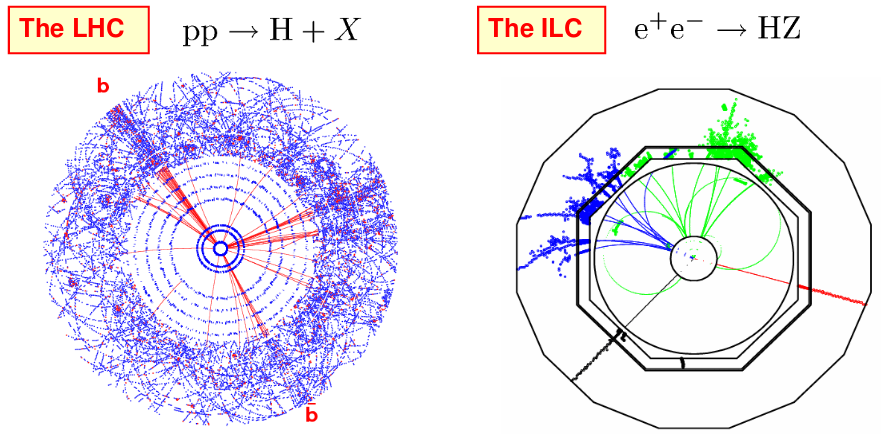
\includegraphics[width=0.5\textwidth]{Figures/Cleanliness.png}
\caption[Clean environment at the ILC]{Comparison of the event displays of a Higgs event at the  LHC and at the ILC.\cite[p. 4]{ILCPhysics_Thomson}\\
The comparison shows that at the ILC the hits recorded are exclusively from the final state particles of the physics interaction.
At the LHC, underlying and pileup events populate the detector.}
\label{fig:Cleanliness}
\end{figure}

\paragraph{Democracy}
Because the elementary coupling e of photons is the same for all quarks and leptons, the \electron \positron annihilation produces pairs of all species, from the Standard Model and Beyond Standard Model, at similar rates.
Besides that, the ILC will be taking data without triggers, i.e. all events will be recorded.
This is possible because of the Cleanliness.
\paragraph{Calculability}
The energies involved in the initial states are precisely known, since there are only point-like elementary particles in initial state.
There are only events with couplings to electroweak interactions.
Additionally, systematic uncertainties due to PDF uncertainties and QCD corrections are omitted.
\paragraph{Detail}
Because of the clean events and the possibility to record and store all taken data, events can be reconstructed in completeness without theoretical assumptions.
The quark and lepton momenta can therefore be determined by kinematic fits.
Studies of the spin-dependence of the production and decay processes are also possible.\\
Due to the high energy resolution and the fact that the initial particle energies are precisely known, particles with small mass differences are distinguishable, i.e. peaks in mass spectra that are close together are more likely to be separable.\\
Additionally, the nano-sized beam of the ILC allows the vertex detector to be close to the IP. 
Hence, c-tagging is possible at the ILC which improves a lot of physics studies.

\subsubsection{ILC as a Higgs factory}
One could call the ILC a Higgs factory, since the total cross section for Higgs production is 10\textsuperscript{-2} in comparison to 10\textsuperscript{-9} for the LHC for example.
%TODO : Find source or plot that shows the total production cross sections at ILC and LHC
Therefore, the number of Higgs events measured at the ILC will be significantly higher, namely about 10 Higgs events per hour.
Due to the large statistics and the capability for precision measurements, the individual Higgs couplings can be measured to a percent accuracy and the global width of the Higgs can be measured directly.
When taking the LHC as an example, the LHC experiments have to make a global fit to all Higgs signals and make assumptions of the Higgs width, in order to get the Higgs couplings.
This can not be as precise as at the ILC, as can be seen in Figure~\ref{fig:Higgs_couplings}.
Only for the coupling to photons, the LHC yields more precise measurements which can only be topped by the combination of the LHC and the ILC results.

\begin{figure}
\centering
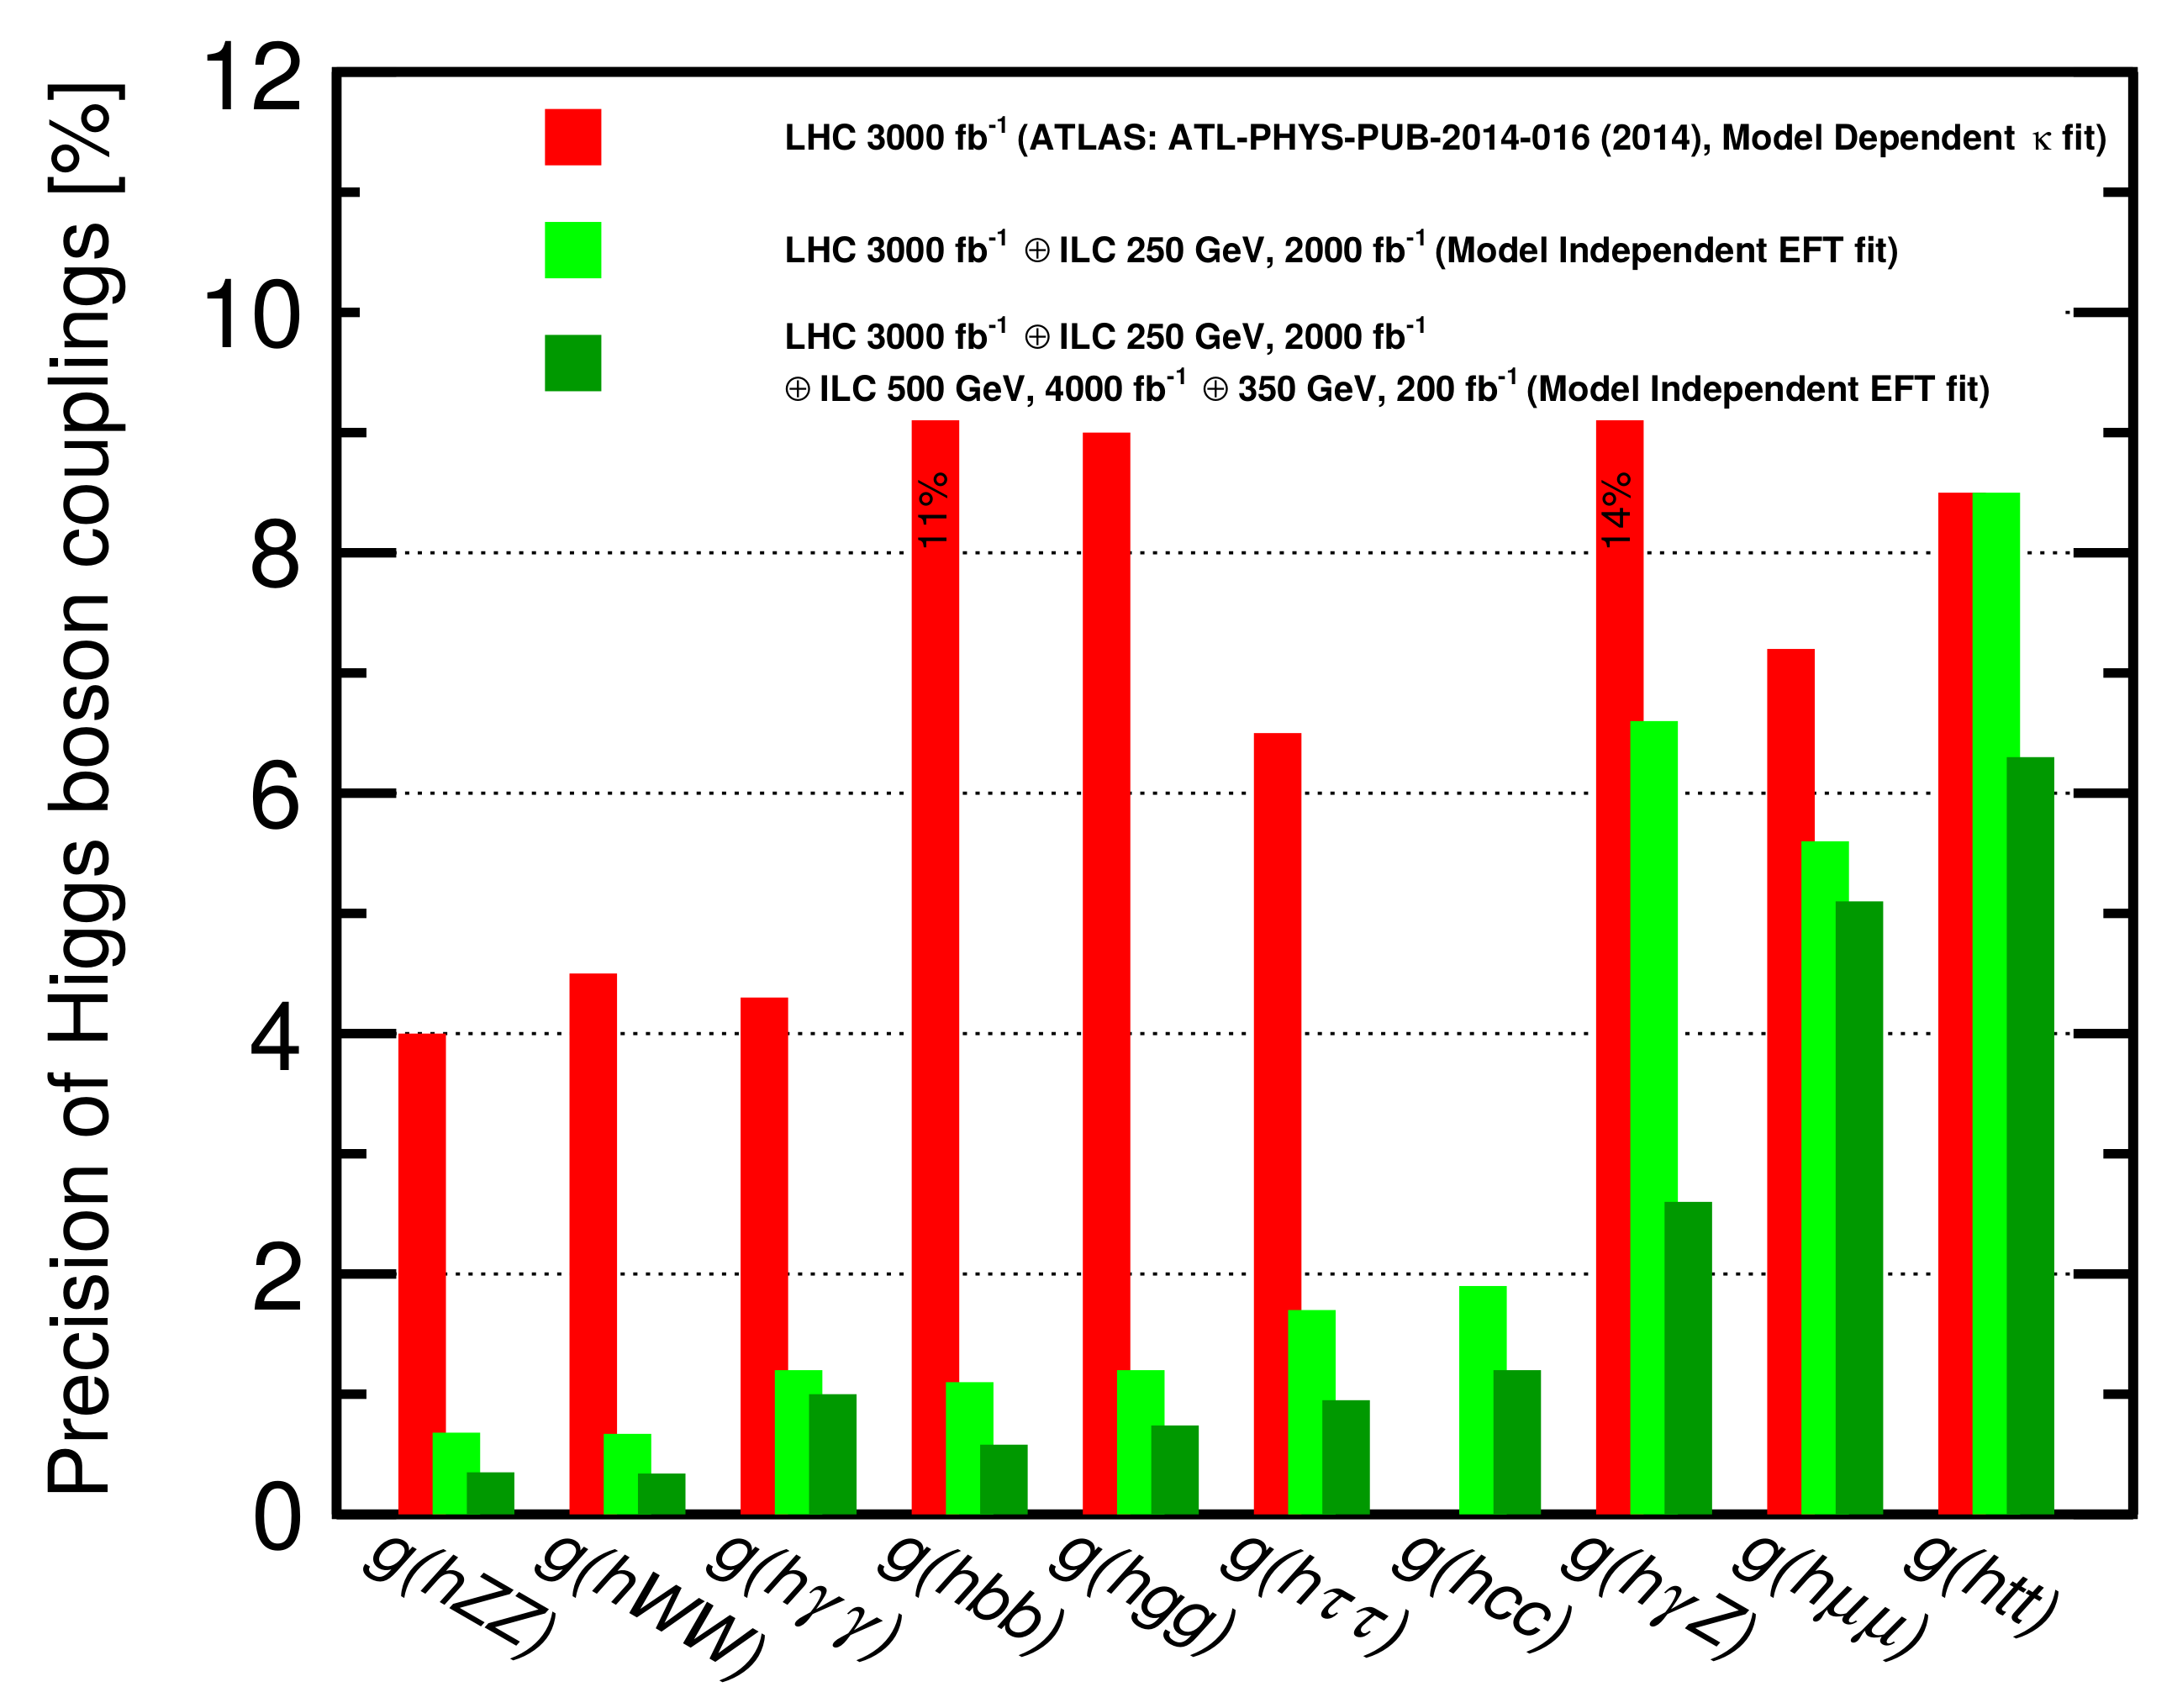
\includegraphics[width=0.5\textwidth]{Figures/Higgs_couplings.png}
\caption[Higgs coupling precisions]{Comparison of the Higgs coupling precision reached at the ILC and at the LHC.\cite[p. 9]{ILCPhysics}\\
The plot shows the relative precisions for the Higgs couplings calculated from the model-dependent fits to simulated data from the High-Luminosity LHC and the ILC.}
\label{fig:Higgs_couplings}
\end{figure}
%TODO : Check if there is a more up-to-date picture

\section{Possible Site}
\label{ILC:site}
Out of originally 10 potential ILC sites in Japan, the Kitakami mountains in the Tohuku Prefecture was chosen to be the preferred site for the ILC.
This decision was made in July 2013 after a detailed study of all site specific factors, like the geological conditions, the infrastructure, and the impact on the environment and the economy.
As can be seen in Figure~\ref{fig:ILC_Site}, the closest city with about 120,000 citizens would be Ichinoseki.
Morioka and Sendai are the biggest cities around the candidate site, with Tokyo being about \SI{430}{\kilo\meter} away.
Although being in the north of Japan, the travel time from Tokyo is only about three hours, and the proximity to the coast line allows the transportation of construction, machine and detector parts by ship.

\begin{figure}
\centering
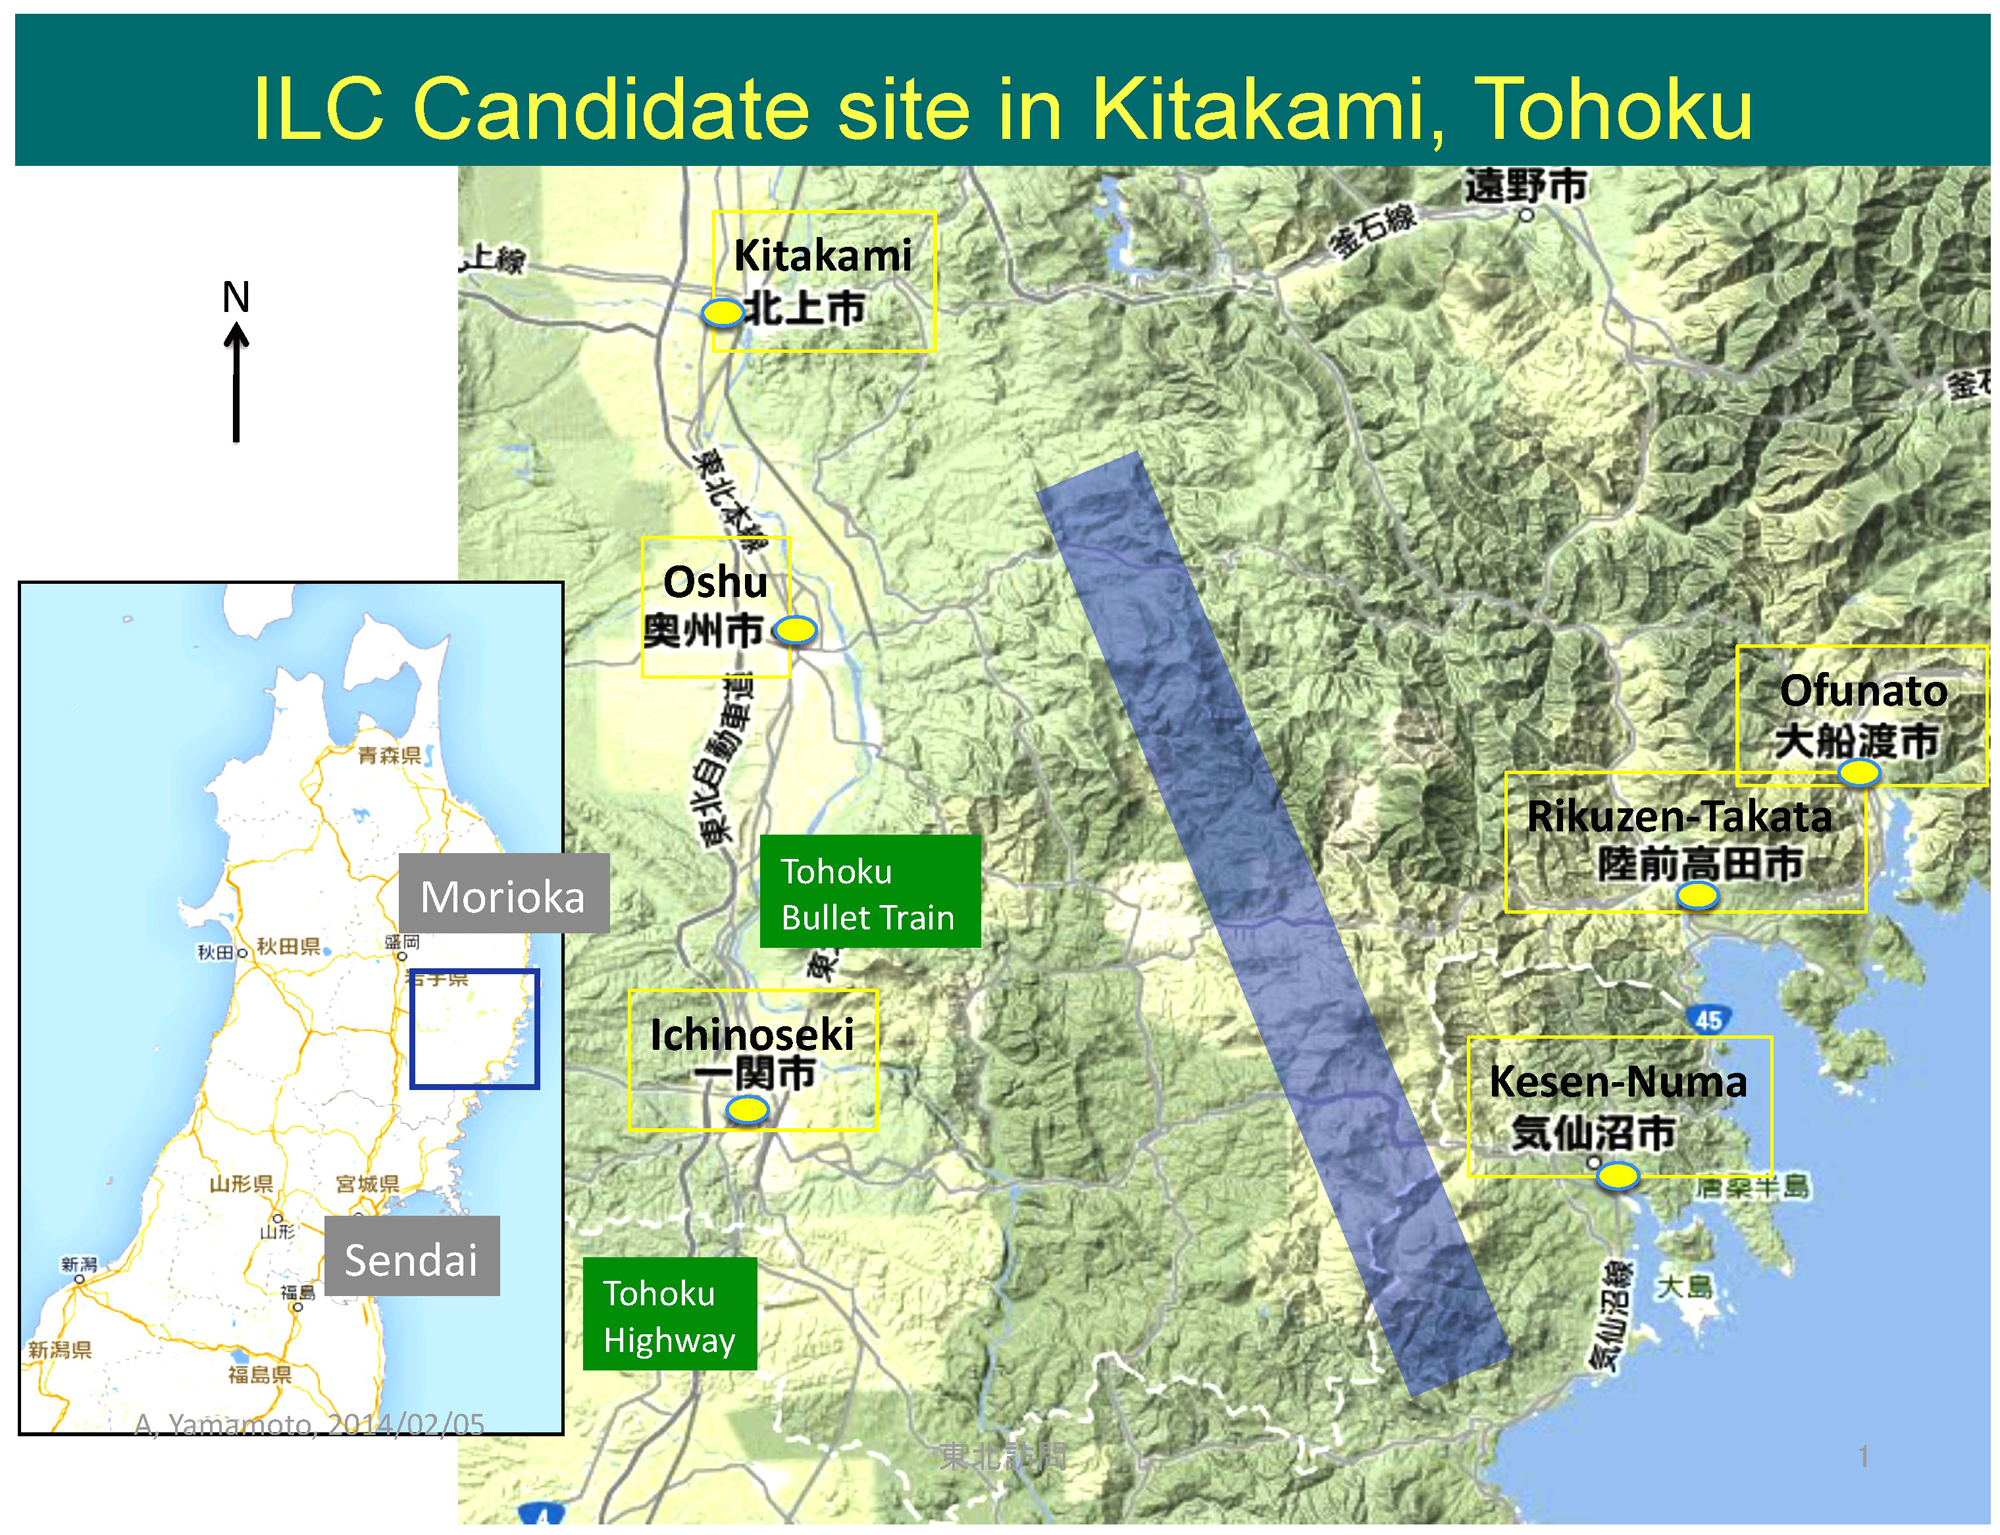
\includegraphics[width=0.6\textwidth]{Figures/ILC-site.jpg}
\caption[Possible site for the ILC]{The possible site for the ILC are the Kitakami mountains in the Tohuku Prefecture.\cite{Site}}
\label{fig:ILC_Site}
\end{figure}

\section{The Experiments}
\label{ILC:detectors}

In order to preserve the competitive spirit and the ability to cross-check results, the ILC has two detectors despite the fact that it is a linear and not a circular collider.
The so-called push-pull system makes that possible by allowing the detectors to switch position after a certain amount of data-taking time.
The whole detector together with the last quadrupole magnet of the accelerator Final Focus system will be pulled out of the beam line, and the other one will be pushed in.
The whole process is designed to take only a short time, i.e. several hours up to 1-2 days, but involves some challenges especially for the magnets, the cryogenics and the detector and machine alignment.\cite[p. 28-29]{TDR1}
The two detectors, the Silicon Detector (SiD) and the International Large Detector (ILD), will be explained in detail in the following with a bigger focus on the SiD detector since some of the background studies presented in the thesis were made for the SiD only.

\subsection{The Silicon Detector}
The SiD is designed to be a robust, compact detector with the vertex and tracker subdetectors and the electromagnetic calorimeter (ECAL) being based on silicon sensors.
The silicon design in comparison to other designs for the vertex and tracking detectors is more robust regarding the beam background and timing.
With also the highly segmented hadronic calorimeter being inside the solenoid field, particle tracking is possible even in the calorimeters.
With being designed to be compact, the measurements for the full detector are \SI{14}{m} in height and \SI{11}{m} in length.
To compensate the small radius, so that SiD is still hermetic and contains the full particle showers, the magnetic field of the superconducting solenoid magnet is \SI{5}{T}.

Figure~\ref{fig:SiD} shows schematic drawings of the SiD detector and its subdetectors.

\begin{figure}
\centering
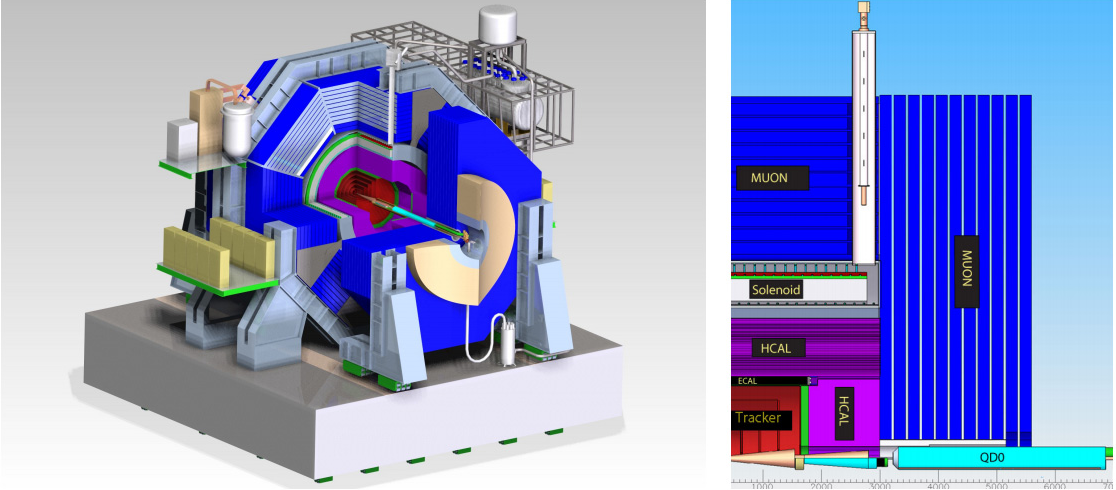
\includegraphics[width=0.7\textwidth]{Figures/SiD.png}
\caption[Schematic drawing of the SiD detector]{The SiD detector consists of the vertex and tracking detectors (red), the electromagnetic calorimeter (ECAL) (green), the hadronic calorimeter (HCAL) (purple) and the muon system (blue). All subdetectors except the muon system are inside the solenoid magnet.\cite[p. 31]{TDR1}}
\label{fig:SiD}
\end{figure}
%TODO : Update the picture of the SiD detector -> new design for muon system

Overall the SiD detector is optimized for Particle Flow Algorithms (PFA).
PFA is a reconstruction method that reconstructs each particle of the final state individually and uses the different subdetectors for a specific purpose.
Therefore, charged particles are reconstructed from tracks in the tracker device, the ECAL is used for photons, and the ECAL and HCAL together for other neutral particles. 
%TODO : Find a source for explanation of PFA

Table~\ref{tab:KeyParametersSiD} lists the key parameters and measurements of the SiD subdetector systems.

\begin{table}
\caption{Key parameters of the baseline SiD design. All dimensions are given in cm.\cite{SiDBkgNote}}
\label{tab:KeyParametersSiD}
\centering
\begin{tabularx}{0.81\textwidth}{l|llll}
\hline\hline
SiD Barrel & Technology & Inner radius & Outer radius & z extent\\
\hline
Vertex detector & Silicon pixels & 1.4 & 6.0 & $\pm 6.25$ \\
Tracker & Silicon strips & 21.7 & 122.1 & $\pm 152.2$ \\
ECAL & Silicon pixels-W & 126.5 & 140.9 & $\pm 176.5$ \\
HCAL & RPC-steel & 141.7 & 249.3 & $\pm 301.8$ \\
Solenoid & 5 T SC & 259.1 & 339.2 & $\pm 298.3$ \\
Flux return & Scintillator-steel & 340.2 & 604.2 & $\pm 303.3$ \\
\hline
SiD Endcap & Technology & Inner z & Outer z & Outer radius\\
\hline
Vertex detector & Silicon pixels & 7.3 & 83.4 & 16.6 \\
Tracker & Silicon strips & 77.0 & 164.3 & 125.5 \\
ECAL & Silicon pixel-W & 165.7 & 180.0 & 125.0 \\
HCAL & RPC-steel & 180.5 & 302.8 & 140.2 \\
Flux return & Scintillator/steel & 303.3 & 567.3 & 604.2 \\
LumiCal & Silicon-W & 155.7 & 169.55 &  20.0 \\
BeamCal & Semiconductor-W & 326.5 & 344 & 14.0 \\
\hline\hline
\end{tabularx}
\end{table}

\subsection{The International Large Detector}

Like the SiD detector, ILD is a multi-purpose particle detector that is optimized for PFA.
Its vertex detector is also based on silicon sensors, whereas the tracker is a combination of both, a silicon strip and pixel detector and a time projection chamber (TPC).
Also similar to SiD, the calorimeters are within the solenoid magnet, which is only surrounded by the muon system.
The magnetic field of the superconducting solenoid magnet is \SI{3.5}{T} for the ILD.
Because of having a big gaseous volume, the full detector is bigger than SiD, namely \SI{16}{m} in height and \SI{14}{m} in length.
Figure~\ref{fig:ILD} shows all the subdetectors mentioned above in two schematic drawings of the ILD detector.

\begin{figure}
\centering
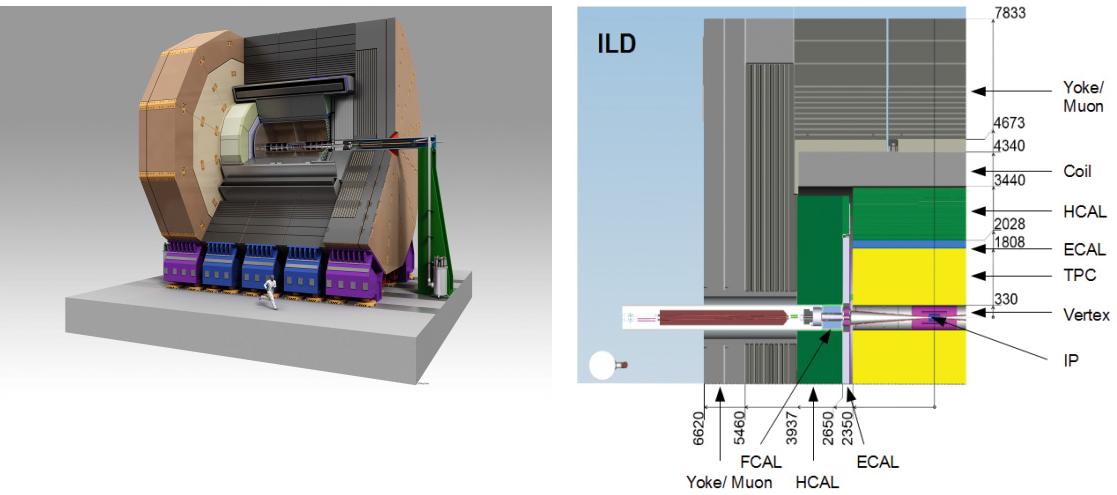
\includegraphics[width=0.7\textwidth]{Figures/ILD.png}
\caption[Schematic drawing of the ILD detector]{The ILD detector consists of the vertex detector (pink), the time projection chamber (TPC) (yellow), the electromagnetic calorimeter (ECAL) (blue), the hadronic calorimeter (HCAL) (green) and the muon system (gray). All subdetectors except the muon system are inside the solenoid magnet.\cite[p. 34]{TDR1}}
\label{fig:ILD}
\end{figure}
%TODO : Check if I have to update the picture of the ILD detector
